% answers.tex —— 2007 年·普通高等学校招生考试·陕西卷·理科 · 参考答案与详细解析片段
% 由 tools/generate_projects.py 依来源总账自 2007/2007_数学真题_陕西理_试题.md + 2007/2007_数学真题_陕西理_解析正文.md + 2007/2007_数学真题_陕西理_答案要点.md 生成，勿手改（改源 MD 后重跑）


\begin{gktip}
固定候选 PDF 仅含题面，无答案、解析和评分标准，原卷亦未标注分值；以下为非官方编者独立推导，官方答案字段为空。来源发布者、出版者、版次与官方身份均未核。
\end{gktip}

\begin{answer}
\gksolhead{1}{}

\textbf{题目}：

在复平面内，复数 $z=\dfrac{1}{2+\mathrm i}$ 对应的点位于（　）

（A）第一象限

（B）第二象限

（C）第三象限

（D）第四象限

\Needspace{4\baselineskip}
\textbf{解析}

\nopagebreak[4]
\[z=\frac1{2+\mathrm i}=\frac{2-\mathrm i}{5}=\frac25-\frac15\mathrm i,\]

对应点 $\left(\dfrac25,-\dfrac15\right)$ 在第四象限。

\gkanswer{答案：D。}

\end{answer}
\begin{answer}
\gksolhead{2}{}

\textbf{题目}：

已知全集 $U=\{1,2,3,4,5\}$，集合 $A=\{x\in\mathbf Z\mid |x-3|<2\}$，则集合 $\complement_UA$ 等于（　）

（A）$\{1,2,3,4\}$

（B）$\{2,3,4\}$

（C）$\{1,5\}$

（D）$\{5\}$

\Needspace{4\baselineskip}
\textbf{解析}

$|x-3|<2\Rightarrow1<x<5$，整数 $x=2,3,4$，故 $A=\{2,3,4\}$，$\complement_UA=\{1,5\}$。

\gkanswer{答案：C。}

\end{answer}
\begin{answer}
\gksolhead{3}{}

\textbf{题目}：

抛物线 $y=x^2$ 的准线方程是（　）

（A）$4y+1=0$

（B）$4x+1=0$

（C）$2y+1=0$

（D）$2x+1=0$

\Needspace{4\baselineskip}
\textbf{解析}

$y=x^2$ 即 $x^2=2py$ 中 $p=\dfrac12$，准线 $y=-\dfrac14$，即 $4y+1=0$。

\gkanswer{答案：A。}

\end{answer}
\begin{answer}
\gksolhead{4}{}

\textbf{题目}：

已知 $\sin\alpha=\dfrac{\sqrt5}{5}$，则 $\sin^4\alpha-\cos^4\alpha$ 的值为（　）

（A）$-\dfrac15$

（B）$-\dfrac35$

（C）$\dfrac15$

（D）$\dfrac35$

\Needspace{4\baselineskip}
\textbf{解析}

\nopagebreak[4]
\[\sin^4\alpha-\cos^4\alpha=2\sin^2\alpha-1=2\cdot\frac15-1=-\frac35.\]

\gkanswer{答案：B。}

\end{answer}
\begin{answer}
\gksolhead{5}{}

\textbf{题目}：

各项均为正数的等比数列 $\{a_n\}$ 的前 $n$ 项和为 $S_n$。若 $S_n=2$，$S_{3n}=14$，则 $S_{4n}$ 等于（　）

（A）$80$

（B）$30$

（C）$26$

（D）$16$

\Needspace{4\baselineskip}
\textbf{解析}

\Needspace{5\baselineskip}
设 $q^n=t>0$。由

\nopagebreak[4]
\[\frac{S_{3n}}{S_n}=1+t+t^2=\frac{14}{2}=7,\]

\Needspace{5\baselineskip}
得 $t^2+t-6=0$，$t=2$。于是

\nopagebreak[4]
\[S_{4n}=S_n(1+t)(1+t^2)=2\times3\times5=30.\]

\gkanswer{答案：B。}

\end{answer}
\begin{answer}
\gksolhead{6}{}

\textbf{题目}：

一个正三棱锥的四个顶点都在半径为 $1$ 的球面上，其中底面的三个顶点在该球的一个大圆上，则该正三棱锥的体积是（　）

（A）$\dfrac{3\sqrt3}{4}$

（B）$\dfrac{\sqrt3}{3}$

（C）$\dfrac{\sqrt3}{4}$

（D）$\dfrac{\sqrt3}{12}$

\Needspace{4\baselineskip}
\textbf{解析}

\Needspace{5\baselineskip}
底面三顶点在大圆上，故底面外接圆半径为 $1$，正三角形边长 $\sqrt3$，面积 $\dfrac{3\sqrt3}{4}$。球心为底面中心，顶点在球面上，高为 $1$。体积

\nopagebreak[4]
\[V=\frac13\cdot\frac{3\sqrt3}{4}\cdot1=\frac{\sqrt3}{4}.\]

\gkanswer{答案：C。}

\end{answer}
\begin{answer}
\gksolhead{7}{}

\textbf{题目}：

已知双曲线 $C$：$\dfrac{x^2}{a^2}-\dfrac{y^2}{b^2}=1$（$a>0$，$b>0$），以 $C$ 的右焦点为圆心且与 $C$ 的渐近线相切的圆的半径是（　）

（A）$\sqrt{ab}$

（B）$\sqrt{a^2+b^2}$

（C）$a$

（D）$b$

\Needspace{4\baselineskip}
\textbf{解析}

\Needspace{5\baselineskip}
右焦点到渐近线 $bx-ay=0$ 的距离为

\nopagebreak[4]
\[\frac{|bc|}{c}=b.\]

\gkanswer{答案：D。}

\end{answer}
\begin{answer}
\gksolhead{8}{}

\textbf{题目}：

若函数 $f(x)$ 的反函数 $f^{-1}(x)$，则函数 $f(x-1)$ 与 $f^{-1}(x-1)$ 的图象可能是（　）
\nopagebreak[4]
\begin{center}% 2007 年陕西卷理科第 8 题：f(x-1) 与 f^{-1}(x-1) 的图象四选项。
%   （D）正确：两曲线关于 y=x-1 对称；其余为平移/对称错误的干扰项。
% 来源 PDF：gaokaomath-src/普通高考/2007/2007陕西理.pdf
% SHA-256：13d2ff59859300ff8372770c8d5877b5b9e8a81f4934dcc5481588f27cf745f7
% 原页：2007陕西理.pdf 第 1 页（A3 三栏）第 1 栏，书页码 401。
% 重绘依据：按原页四个小图的曲线、渐近线与对称关系重绘。
\begin{tikzpicture}[scale=0.8, semithick,
  every node/.style={inner sep=1pt, font=\small}]
  % A
  \begin{scope}[shift={(0,0)}]
    \draw[->,>=stealth] (-0.5,0) -- (2.7,0) node[right] {$x$};
    \draw[->,>=stealth] (0,-0.5) -- (0,2.2) node[above] {$y$};
    \draw[domain=0:1.5,samples=60] plot (\x,{0.6*exp(0.8*\x)});
    \draw[domain=0.2:2.5,samples=60] plot (\x,{0.5*exp(0.8*(\x-1))});
    \node[below] at (1,-0.8) {（A）};
  \end{scope}
  % B
  \begin{scope}[shift={(4.4,0)}]
    \draw[->,>=stealth] (-0.5,0) -- (2.7,0) node[right] {$x$};
    \draw[->,>=stealth] (0,-0.5) -- (0,2.2) node[above] {$y$};
    \draw[domain=0:1.6,samples=60] plot (\x,{0.5*exp(0.9*\x)});
    \draw[domain=1.05:2.5,samples=60] plot (\x,{ln(\x-1)/ln(2)+1});
    \node[below] at (1,-0.8) {（B）};
  \end{scope}
  % C
  \begin{scope}[shift={(0,-4.2)}]
    \draw[->,>=stealth] (-0.5,0) -- (2.7,0) node[right] {$x$};
    \draw[->,>=stealth] (0,-0.5) -- (0,2.2) node[above] {$y$};
    \draw[domain=0.2:2.5,samples=60] plot (\x,{ln(\x)/ln(2)+0.6});
    \draw[domain=1.05:2.5,samples=60] plot (\x,{ln(\x-1)/ln(2)});
    \node[below] at (1,-0.8) {（C）};
  \end{scope}
  % D 正确
  \begin{scope}[shift={(4.4,-4.2)}]
    \draw[->,>=stealth] (-0.5,0) -- (2.7,0) node[right] {$x$};
    \draw[->,>=stealth] (0,-0.5) -- (0,2.2) node[above] {$y$};
    \draw[domain=0:1.6,samples=60] plot (\x,{0.55*exp(0.9*\x)});
    \draw[domain=1.05:2.5,samples=60] plot (\x,{ln(\x-1)/ln(2)+1});
    \node[below] at (1,-0.8) {（D）};
  \end{scope}
\end{tikzpicture}
\end{center}
\nopagebreak[4]
\Needspace{4\baselineskip}
\textbf{解析}

$f(x-1)$ 与 $f^{-1}(x-1)$ 的图象关于直线 $y=x-1$ 对称。逐图检查，只有 D 的两条曲线关于该直线对称。

\gkanswer{答案：D。}

\end{answer}
\begin{answer}
\gksolhead{9}{}

\textbf{题目}：

给出如下三个命题：

① 四个非零实数 $a$，$b$，$c$，$d$ 依次成等比数列的充要条件是 $ad=bc$；

② 设 $a$，$b\in\mathbf R$，且 $ab\neq0$，若 $\dfrac ab<1$，则 $\dfrac ba>1$；

③ 若 $f(x)=\log_2x$，则 $f(|x|)$ 是偶函数。

其中不正确的序号是（　）

（A）①②③

（B）①②

（C）②③

（D）①③

\Needspace{4\baselineskip}
\textbf{解析}

① $ad=bc$ 不足以保证依次成等比（如 $1,2,2,4$），不正确；② 若 $a/b<1$ 且 $a,b$ 异号，则 $b/a<0<1$，不正确；③ $f(|x|)=\log_2|x|$ 为偶函数，正确。故不正确的为①②。

\gkanswer{答案：B。}

\end{answer}
\begin{answer}
\gksolhead{10}{}

\textbf{题目}：

已知平面 $\alpha\parallel$ 平面 $\beta$，直线 $m\subset\alpha$，直线 $n\subset\beta$，点 $A\in m$，点 $B\in n$，记点 $A$，$B$ 之间的距离为 $a$，点 $A$ 到直线 $n$ 的距离为 $b$，直线 $m$ 和 $n$ 的距离为 $c$，则（　）

（A）$b\leqslant c\leqslant a$

（B）$a\leqslant c\leqslant b$

（C）$c\leqslant a\leqslant b$

（D）$c\leqslant b\leqslant a$

\Needspace{4\baselineskip}
\textbf{解析}

\Needspace{5\baselineskip}
两平行平面间的距离为 $c$，故 $c\leqslant b$（$A$ 到 $\beta$ 内直线 $n$ 的距离不小于平面间距离），且 $c\leqslant a$。又 $B\in n$，故 $A$ 到 $n$ 的距离不超过 $AB=a$，即 $b\leqslant a$。故

\nopagebreak[4]
\[c\leqslant b\leqslant a.\]

\gkanswer{答案：D。}

\end{answer}
\begin{answer}
\gksolhead{11}{}

\textbf{题目}：

$f(x)$ 是定义在 $(0,+\infty)$ 上的非负可导函数，且满足 $xf'(x)+f(x)\leqslant0$。对任意正数 $a$，$b$，若 $a<b$，则必有（　）

（A）$af(b)\leqslant bf(a)$

（B）$bf(a)\leqslant af(b)$

（C）$af(a)\leqslant f(b)$

（D）$bf(b)\leqslant f(a)$

\Needspace{4\baselineskip}
\textbf{解析}

\nopagebreak[4]
\[(xf(x))'=xf'(x)+f(x)\leqslant0,\]

\Needspace{5\baselineskip}
故 $xf(x)$ 在 $(0,+\infty)$ 上递减。由 $a<b$ 得

\nopagebreak[4]
\[bf(b)\leqslant af(a).\]

\Needspace{5\baselineskip}
又 $\dfrac{f(x)}x$ 的导数

\nopagebreak[4]
\[\left(\frac fx\right)'=\frac{xf'-f}{x^2}\leqslant\frac{-2f}{x^2}\leqslant0,\]

\Needspace{5\baselineskip}
故 $\dfrac{f(x)}x$ 递减，$a<b$ 时

\nopagebreak[4]
\[\frac{f(b)}b\leqslant\frac{f(a)}a\ \Rightarrow\ af(b)\leqslant bf(a).\]

\gkanswer{答案：A。}

\end{answer}
\begin{answer}
\gksolhead{12}{}

\textbf{题目}：

设集合 $S=\{A_0,A_1,A_2,A_3\}$，在 $S$ 上定义运算 $\oplus$ 为：$A_i\oplus A_j=A_k$，其中 $k$ 为 $i+j$ 被 $4$ 除的余数，$i,j=0,1,2,3$。则满足关系式 $(x\oplus x)\oplus A_2=A_0$ 的 $x$（$x\in S$）的个数为（　）

（A）$4$

（B）$3$

（C）$2$

（D）$1$

\Needspace{4\baselineskip}
\textbf{解析}

\Needspace{5\baselineskip}
$x=A_i$ 时 $x\oplus x=A_{2i\bmod4}$，故

\nopagebreak[4]
\[(x\oplus x)\oplus A_2=A_{(2i+2)\bmod4}.\]

要求 $2i+2\equiv0\pmod4$，即 $2i\equiv2\pmod4$，$i=1,3$。共 $2$ 个。

\gkanswer{答案：C。}

\end{answer}
\begin{answer}
\gksolhead{13}{}

\textbf{题目}：

$\lim\limits_{x\to1}\left(\dfrac{2x+1}{x^2+x-2}-\dfrac1{x-1}\right)=$\gkblank{}。

\Needspace{4\baselineskip}
\textbf{解析}

\nopagebreak[4]
\[\frac{2x+1}{x^2+x-2}-\frac1{x-1}
=\frac{2x+1-(x+2)}{(x-1)(x+2)}
=\frac{x-1}{(x-1)(x+2)}=\frac1{x+2},\]

极限为 $\dfrac13$。

\gkanswer{答案：$\dfrac13$。}

\end{answer}
\begin{answer}
\gksolhead{14}{}

\textbf{题目}：

已知实数 $x$，$y$ 满足条件 $\begin{cases}x-2y+4\geqslant0,\\ 2x+y-2\geqslant0,\\ 3x-y-3\leqslant0,\end{cases}$ 则 $z=x+2y$ 的最大值为\gkblank{}。

\Needspace{4\baselineskip}
\textbf{解析}

\Needspace{5\baselineskip}
可行域顶点为 $(0,2)$，$(1,0)$，$(2,3)$。计算

\nopagebreak[4]
\[z=x+2y:\quad4,\ 1,\ 8,\]

最大值为 $8$。

\gkanswer{答案：$8$。}

\end{answer}
\begin{answer}
\gksolhead{15}{}

\textbf{题目}：

如图，平面内有三个向量 $\overrightarrow{OA}$，$\overrightarrow{OB}$，$\overrightarrow{OC}$，其中 $\overrightarrow{OA}$ 与 $\overrightarrow{OB}$ 的夹角为 $120^\circ$，$\overrightarrow{OA}$ 与 $\overrightarrow{OC}$ 的夹角为 $30^\circ$，且 $|\overrightarrow{OA}|=|\overrightarrow{OB}|=1$，$|\overrightarrow{OC}|=2\sqrt3$。若 $\overrightarrow{OC}=\lambda\overrightarrow{OA}+\mu\overrightarrow{OB}$（$\lambda$，$\mu\in\mathbf R$），则 $\lambda+\mu$ 的值为\gkblank{}。
\nopagebreak[4]
\begin{center}% 2007 年陕西卷理科第 15 题：向量 OA、OB、OC 的夹角关系。
%   OA 与 OB 成 120°，OA 与 OC 成 30°，|OA|=|OB|=1，|OC|=2√3。
% 来源 PDF：gaokaomath-src/普通高考/2007/2007陕西理.pdf
% SHA-256：95abaa3050f33e9b9587ad186af8f173fbf40c31ebe3f2be710bbae607ed0ecb
% 原页：2007陕西理.pdf 第 1 页（A3 三栏）第 3 栏，书页码 401。
% 重绘依据：按原页三个向量的方向与长度比例重绘。
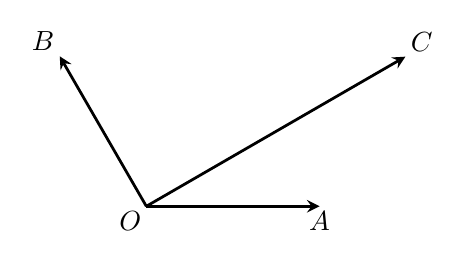
\begin{tikzpicture}[scale=1.0, semithick,
  every node/.style={inner sep=1.5pt}]
  \coordinate (O) at (0,0);
  \coordinate (A) at (2.2,0);
  \coordinate (B) at (-1.1,1.905);
  \coordinate (C) at (3.29,1.9);

  \draw[->,>=stealth,line width=1pt] (O) -- (A) node[below] {$A$};
  \draw[->,>=stealth,line width=1pt] (O) -- (B) node[above left] {$B$};
  \draw[->,>=stealth,line width=1pt] (O) -- (C) node[above right] {$C$};
  \node[below left] at (O) {$O$};
\end{tikzpicture}
\end{center}
\nopagebreak[4]
\Needspace{4\baselineskip}
\textbf{解析}

同文科卷第 16 题，由点积方程得 $\lambda=4$，$\mu=2$，故 $\lambda+\mu=6$。

\gkanswer{答案：$6$。}

\end{answer}
\begin{answer}
\gksolhead{16}{}

\textbf{题目}：

安排 $3$ 名支教教师去 $6$ 所学校任教，每校至多 $2$ 人，则不同的分配方案共有\gkblank{}种。（用数字作答）

\Needspace{4\baselineskip}
\textbf{解析}

\Needspace{5\baselineskip}
不加限制共有 $6^3=216$ 种；某校分到 $3$ 人的情况有 $6$ 种。故

\nopagebreak[4]
\[216-6=210.\]

\gkanswer{答案：$210$。}

\end{answer}
\begin{answer}
\gksolhead{17}{}

\textbf{题目}：

设函数 $f(x)=\boldsymbol a\cdot\boldsymbol b$，其中向量 $\boldsymbol a=(m,\cos2x)$，$\boldsymbol b=(1+\sin2x,1)$，$x\in\mathbf R$，且函数 $y=f(x)$ 的图象经过点 $\left(\dfrac{\pi}{4},2\right)$。

（1）求实数 $m$ 的值；

（2）求函数 $f(x)$ 的最小值及此时 $x$ 值的集合。

\Needspace{4\baselineskip}
\textbf{解析}

\Needspace{5\baselineskip}
（1）$f(x)=m(1+\sin2x)+\cos2x$。由 $f\left(\dfrac{\pi}{4}\right)=2$：

\nopagebreak[4]
\[m(1+1)+0=2\ \Rightarrow\ m=1.\]

\Needspace{5\baselineskip}
（2）

\nopagebreak[4]
\[f(x)=1+\sin2x+\cos2x=1+\sqrt2\sin\left(2x+\frac{\pi}{4}\right),\]

\Needspace{5\baselineskip}
最小值为 $1-\sqrt2$，当

\nopagebreak[4]
\[2x+\frac{\pi}{4}=-\frac{\pi}{2}+2k\pi\ \Rightarrow\ x=-\frac{3\pi}{8}+k\pi.\]

\gkanswer{答案：（1）$m=1$；（2）最小值 $1-\sqrt2$，此时 $x=-\dfrac{3\pi}{8}+k\pi$（$k\in\mathbf Z$）。}

\end{answer}
\begin{answer}
\gksolhead{18}{}

\textbf{题目}：

某项选拔共有三轮考核，每轮设有一个问题，能正确回答问题者进入下一轮考核，否则即被淘汰。已知某选手能正确回答第一、二、三轮的问题的概率分别为 $\dfrac45$，$\dfrac35$，$\dfrac25$，且各轮问题能否正确回答互不影响。

（1）求该选手被淘汰的概率；

（2）该选手在选拔中回答问题的个数记为 $\xi$，求随机变量 $\xi$ 的分布列与数学期望。

\Needspace{4\baselineskip}
\textbf{解析}

\Needspace{5\baselineskip}
（1）不被淘汰即三轮全对：

\nopagebreak[4]
\[P=\frac45\cdot\frac35\cdot\frac25=\frac{24}{125},\]

\Needspace{5\baselineskip}
故被淘汰概率

\nopagebreak[4]
\[1-\frac{24}{125}=\frac{101}{125}.\]

（2）$\xi=1$：第一轮失败，$P=\dfrac15$；

$\xi=2$：第一轮通过、第二轮失败，$P=\dfrac45\cdot\dfrac25=\dfrac8{25}$；

$\xi=3$：前两轮通过，$P=\dfrac45\cdot\dfrac35=\dfrac{12}{25}$。

分布列：

\begin{center}
\begin{tabular}{llll}
\toprule
$\xi$ & 1 & 2 & 3 \\
\midrule
$P$ & $\frac15$ & $\frac8{25}$ & $\frac{12}{25}$ \\
\bottomrule
\end{tabular}
\end{center}

\nopagebreak[4]
\[E\xi=1\cdot\frac15+2\cdot\frac8{25}+3\cdot\frac{12}{25}
=\frac{5+16+36}{25}=\frac{57}{25}.\]

\gkanswer{答案：（1）$\dfrac{101}{125}$；（2）分布列见解析，$E\xi=\dfrac{57}{25}$。}

\end{answer}
\begin{answer}
\gksolhead{19}{}

\textbf{题目}：

如图，在底面为直角梯形的四棱锥 $P-ABCD$ 中，$AD\parallel BC$，$\angle ABC=90^\circ$，$PA\perp$ 平面 $ABCD$，$PA=4$，$AD=2$，$AB=2\sqrt3$，$BC=6$。

（1）求证：$BD\perp$ 平面 $PAC$；

（2）求二面角 $A-PC-D$ 的大小。
\nopagebreak[4]
\begin{center}% 2007 年陕西卷理科第 19 题：底面为直角梯形的四棱锥 P-ABCD，PA⊥底面。
%   AD∥BC，∠ABC=90°，PA=3，AD=2，AB=2√3，BC=6；E 为 AC 与 BD 的交点。
% 来源 PDF：gaokaomath-src/普通高考/2007/2007陕西理.pdf
% SHA-256：95abaa3050f33e9b9587ad186af8f173fbf40c31ebe3f2be710bbae607ed0ecb
% 原页：2007陕西理.pdf 第 2 页（A3 三栏）第 1 栏，书页码 402。
% 重绘依据：按原页底面梯形、P 的位置与 E 点重绘。
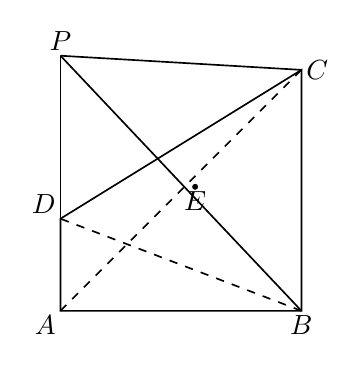
\begin{tikzpicture}[scale=0.9, semithick,
  every node/.style={inner sep=1.5pt}]
  \coordinate (A) at (0,0);
  \coordinate (B) at (3.4,0);
  \coordinate (C) at (3.4,3.4);
  \coordinate (D) at (0,1.3);
  \coordinate (P) at (0,3.6);
  \coordinate (E) at (1.9,1.75);

  \draw (A) -- (B) -- (C) -- (D) -- cycle;
  \draw (P) -- (A);
  \draw (P) -- (B);
  \draw (P) -- (C);
  \draw (P) -- (D);
  \draw[dashed] (A) -- (C);
  \draw[dashed] (B) -- (D);
  \fill (E) circle (1.2pt);

  \node[below left] at (A) {$A$};
  \node[below] at (B) {$B$};
  \node[right] at (C) {$C$};
  \node[above left] at (D) {$D$};
  \node[above] at (P) {$P$};
  \node[below] at (E) {$E$};
\end{tikzpicture}
\end{center}
\nopagebreak[4]
\Needspace{4\baselineskip}
\textbf{解析}

\Needspace{5\baselineskip}
以 $A$ 为原点，$AB$，$AD$，$AP$ 为 $x$，$y$，$z$ 轴：

\nopagebreak[4]
\[A(0,0,0),\ B(2\sqrt3,0,0),\ C(2\sqrt3,6,0),\ D(0,2,0),\ P(0,0,4).\]

（1）$\overrightarrow{BD}=(-2\sqrt3,2,0)$，$\overrightarrow{AC}=(2\sqrt3,6,0)$，点积为 $0$，故 $BD\perp AC$；又 $PA\perp$ 底面，$PA\perp BD$，故 $BD\perp$ 平面 $PAC$。

\Needspace{5\baselineskip}
（2）平面 $APC$ 内

\nopagebreak[4]
\[\overrightarrow{AP}=(0,0,4),\qquad \overrightarrow{AC}=(2\sqrt3,6,0),\]

\Needspace{5\baselineskip}
法向量

\nopagebreak[4]
\[\boldsymbol n_1=(-24,8\sqrt3,0)\sim(-3,\sqrt3,0).\]

\Needspace{5\baselineskip}
平面 $PCD$ 内

\nopagebreak[4]
\[\overrightarrow{PC}=(2\sqrt3,6,-4),\qquad \overrightarrow{PD}=(0,2,-4),\]

\Needspace{5\baselineskip}
法向量

\nopagebreak[4]
\[\boldsymbol n_2=(-16,8\sqrt3,4\sqrt3)\sim(-4,2\sqrt3,\sqrt3).\]

\Needspace{5\baselineskip}
设二面角为 $\theta$，则

\nopagebreak[4]
\[\cos\theta=\frac{|\boldsymbol n_1\cdot\boldsymbol n_2|}{|\boldsymbol n_1||\boldsymbol n_2|}
=\frac{18}{2\sqrt3\cdot\sqrt{31}}=\frac9{\sqrt{93}}.\]

故 $\theta=\arccos\dfrac9{\sqrt{93}}$。

\gkanswer{答案：（1）证明见解析；（2）$\arccos\dfrac{9}{\sqrt{93}}$。}

\end{answer}
\begin{answer}
\gksolhead{20}{}

\textbf{题目}：

设函数 $f(x)=\dfrac{\mathrm e^x}{x^2+ax+a}$，其中 $a$ 为实数。

（1）若 $f(x)$ 的定义域为 $\mathbf R$，求 $a$ 的取值范围；

（2）当 $f(x)$ 的定义域为 $\mathbf R$ 时，求 $f(x)$ 的单调减区间。

\Needspace{4\baselineskip}
\textbf{解析}

\Needspace{5\baselineskip}
（1）定义域为 $\mathbf R$ 需分母恒正：

\nopagebreak[4]
\[\Delta=a^2-4a<0\ \Rightarrow\ 0<a<4.\]

\Needspace{5\baselineskip}
（2）

\nopagebreak[4]
\[f'(x)=\frac{\mathrm e^x(x^2+ax+a)-\mathrm e^x(2x+a)}{(x^2+ax+a)^2}
=\frac{\mathrm e^x x(x+a-2)}{(x^2+ax+a)^2}.\]

故减区间由 $x(x+a-2)<0$ 决定：

\begin{itemize}
\item $0<a<2$：减区间 $(0,2-a)$；
\item $a=2$：$x^2\ge0$，无减区间；
\item $2<a<4$：减区间 $(2-a,0)$。
\end{itemize}

\gkanswer{答案：（1）$0<a<4$；（2）见解析。}

\end{answer}
\begin{answer}
\gksolhead{21}{}

\textbf{题目}：

已知椭圆 $C$：$\dfrac{x^2}{a^2}+\dfrac{y^2}{b^2}=1$（$a>b>0$）的离心率为 $\dfrac{\sqrt6}{3}$，短轴一个端点到右焦点的距离为 $\sqrt3$。

（1）求椭圆 $C$ 的方程；

（2）设直线 $l$ 与椭圆 $C$ 交于 $A$，$B$ 两点，坐标原点 $O$ 到直线 $l$ 的距离为 $\dfrac{\sqrt3}{2}$，求 $\triangle AOB$ 面积的最大值。

\Needspace{4\baselineskip}
\textbf{解析}

\Needspace{5\baselineskip}
（1）短轴端点到右焦点距离为 $\sqrt{b^2+c^2}=a=\sqrt3$。又

\nopagebreak[4]
\[e=\frac ca=\frac{\sqrt6}{3}\ \Rightarrow\ c=\sqrt2,\]

\nopagebreak[4]
\[b^2=a^2-c^2=3-2=1.\]

\Needspace{5\baselineskip}
故椭圆为

\nopagebreak[4]
\[\frac{x^2}{3}+y^2=1.\]

\Needspace{5\baselineskip}
（2）设 $O$ 到 $l$ 的距离 $d=\dfrac{\sqrt3}{2}$，$l$ 的法线方向角为 $\theta$。弦长

\nopagebreak[4]
\[L=\frac{2ab\sqrt{a^2\sin^2\theta+b^2\cos^2\theta-d^2}}{a^2\sin^2\theta+b^2\cos^2\theta}.\]

\Needspace{5\baselineskip}
令 $A=1+2\sin^2\theta\in[1,3]$，则 $a^2=3$，$b^2=1$，

\nopagebreak[4]
\[L=\frac{2\sqrt3\sqrt{A-\frac34}}{A},\]

\Needspace{5\baselineskip}
面积

\nopagebreak[4]
\[S=\frac12Ld=\frac32\cdot\frac{\sqrt{A-\frac34}}A.\]

\Needspace{5\baselineskip}
设 $g(A)=\dfrac{A-\frac34}{A^2}$，$g'(A)=\dfrac{\frac32A-A^2}{A^4}$，故 $A=\dfrac32$ 时最大，$g=\dfrac13$，

\nopagebreak[4]
\[S_{\max}=\frac32\sqrt{\frac13}=\frac{\sqrt3}{2}.\]

\gkanswer{答案：（1）$\dfrac{x^2}{3}+y^2=1$；（2）$\dfrac{\sqrt3}{2}$。}

\end{answer}
\begin{answer}
\gksolhead{22}{}

\textbf{题目}：

已知各项全不为零的数列 $\{a_k\}$ 的前 $k$ 项和为 $S_k$，且 $S_k=\dfrac12a_ka_{k+1}$（$k\in\mathbf N^*$），其中 $a_1=1$。

（1）求数列 $\{a_k\}$ 的通项公式；

（2）对任意给定的正整数 $n$（$n\geqslant2$），数列 $\{b_k\}$ 满足 $\dfrac{b_{k+1}}{b_k}=\dfrac{k-n}{a_{k+1}}$（$k=1,2,\cdots,n-1$），$b_1=1$。求 $b_1+b_2+\cdots+b_n$。

\Needspace{4\baselineskip}
\textbf{解析}

（1）$k=1$ 时 $S_1=1=\dfrac12a_1a_2=\dfrac12a_2$，故 $a_2=2$。

\Needspace{5\baselineskip}
$k\geqslant2$ 时，

\nopagebreak[4]
\[a_k=S_k-S_{k-1}=\frac12(a_ka_{k+1}-a_{k-1}a_k)=\frac{a_k}2(a_{k+1}-a_{k-1}),\]

\Needspace{5\baselineskip}
因 $a_k\neq0$，得

\nopagebreak[4]
\[a_{k+1}-a_{k-1}=2.\]

\Needspace{5\baselineskip}
故奇数项 $1,3,5,\cdots$，偶数项 $2,4,6,\cdots$，即

\nopagebreak[4]
\[a_k=k.\]

\Needspace{5\baselineskip}
（2）由 $\dfrac{b_{k+1}}{b_k}=\dfrac{k-n}{k+1}$，

\nopagebreak[4]
\[b_k=\prod_{j=1}^{k-1}\frac{j-n}{j+1}
=\frac{(-1)^{k-1}(n-1)(n-2)\cdots(n-k+1)}{k!}
=\frac{(-1)^{k-1}}k\mathrm C_{n-1}^{k-1}.\]

\Needspace{5\baselineskip}
于是

\nopagebreak[4]
\[\sum_{k=1}^n b_k=\sum_{k=1}^n\frac{(-1)^{k-1}}k\mathrm C_{n-1}^{k-1}.\]

\Needspace{5\baselineskip}
利用恒等式

\nopagebreak[4]
\[\sum_{k=1}^n\frac{(-1)^{k-1}}k\mathrm C_{n-1}^{k-1}=\frac1n,\]

\Needspace{5\baselineskip}
故

\nopagebreak[4]
\[b_1+b_2+\cdots+b_n=\frac1n.\]

\gkanswer{答案：（1）$a_k=k$；（2）$\dfrac1n$。}

\end{answer}